\section{Verossimilhança Gaussiana e Atividade}

\begin{frame}{Modelagem de Dados Contínuos: A Normal}
    \begin{itemize}
        \item Para dados contínuos, a verossimilhança é formulada utilizando a \textbf{Função de Densidade de Probabilidade} ($PDF$).
        \item Assumimos que a nossa amostra segue uma distribuição Normal $N(\mu, \sigma^2)$:
        $$f(x_i | \mu, \sigma^2) = \frac{1}{\sqrt{2\pi\sigma^2}} \exp\left(-\frac{(x_i - \mu)^2}{2\sigma^2}\right)$$
        \item Onde $\mu$ é a \textbf{Média Populacional} e $\sigma^2$ é a \textbf{Variância Populacional}.
        \item A verossimilhança conjunta para $N$ observações independentes é dada pelo produtório:
        $$L(\mu, \sigma^2) = \prod_{i=1}^N f(x_i | \mu, \sigma^2) = \prod_{i=1}^N \frac{1}{\sqrt{2\pi\sigma^2}} \exp\left(-\frac{(x_i - \mu)^2}{2\sigma^2}\right)$$
        $$L(\mu, \sigma^2) = \left(2\pi\sigma^2\right)^{-N/2} \exp\left(-\frac{1}{2\sigma^2} \sum_{i=1}^N (x_i - \mu)^2\right)$$
    \end{itemize}
\end{frame}

\begin{frame}{A Log-Verossimilhança Gaussiana}
    \begin{itemize}
        \item Aplicando a transformação logarítmica natural ($\ln$) à verossimilhança Normal:
        $$\ln L(\mu, \sigma^2) = \ln \left[ \left(2\pi\sigma^2\right)^{-N/2} \exp\left(-\frac{1}{2\sigma^2} \sum_{i=1}^N (x_i - \mu)^2\right) \right]$$
        $$\ln L(\mu, \sigma^2) = -\frac{N}{2} \ln(2\pi\sigma^2) - \frac{1}{2\sigma^2} \sum_{i=1}^N (x_i - \mu)^2$$
        \item \textbf{A Conexão com Mínimos Quadrados:}
        \begin{itemize}
            \item Para maximizar a verossimilhança com relação à média $\mu$, a primeira parcela é constante.
            \item Portanto, devemos **maximizar** a segunda parcela, o que equivale a **minimizar** o somatório $\sum_{i=1}^N (x_i - \mu)^2$.
            \item Esse somatório é exatamente a soma dos erros quadráticos!
        \end{itemize}
    \end{itemize}
\end{frame}

\begin{frame}{Estimadores de Máxima Verossimilhança}
    \begin{itemize}
        \item Derivando a log-verossimilhança com relação a $\mu$ e igualando a zero:
        $$\frac{\partial \ln L}{\partial \mu} = \frac{1}{\sigma^2} \sum_{i=1}^N (x_i - \mu) = 0 \implies \hat{\mu}_{MLE} = \frac{1}{N}\sum_{i=1}^N x_i = \bar{X}$$
        \item Derivando com relação a $\sigma^2$ e igualando a zero:
        $$\frac{\partial \ln L}{\partial (\sigma^2)} = -\frac{N}{2\sigma^2} + \frac{1}{2(\sigma^2)^2} \sum_{i=1}^N (x_i - \mu)^2 = 0 \implies \hat{\sigma}^2_{MLE} = \frac{1}{N}\sum_{i=1}^N (x_i - \bar{X})^2$$
        \item \textbf{Nota Importante:}
        O estimador de máxima verossimilhança da variância divide por $N$ e não por $N - 1$. Isso o torna ligeiramente viesado para pequenas amostras.
    \end{itemize}
\end{frame}

\begin{frame}{Visualizando a Log-Verossimilhança Normal}
    \begin{columns}
        \begin{column}{0.5\textwidth}
            \textbf{Análise da Média Amostral:}
            \begin{itemize}
                \item Utilizando a amostra de 170 medições de sala.
                \item Mantemos o desvio padrão constante no seu valor ótimo $\hat{\sigma} \approx 16.6020$.
                \item Avaliamos diferentes médias candidatas $\mu$.
                \item A log-verossimilhança Gaussiana atinge o seu valor máximo exatamente em:
                $$\hat{\mu}_{MLE} = 46.5412$$
            \end{itemize}
        \end{column}
        \begin{column}{0.5\textwidth}
            \centering
            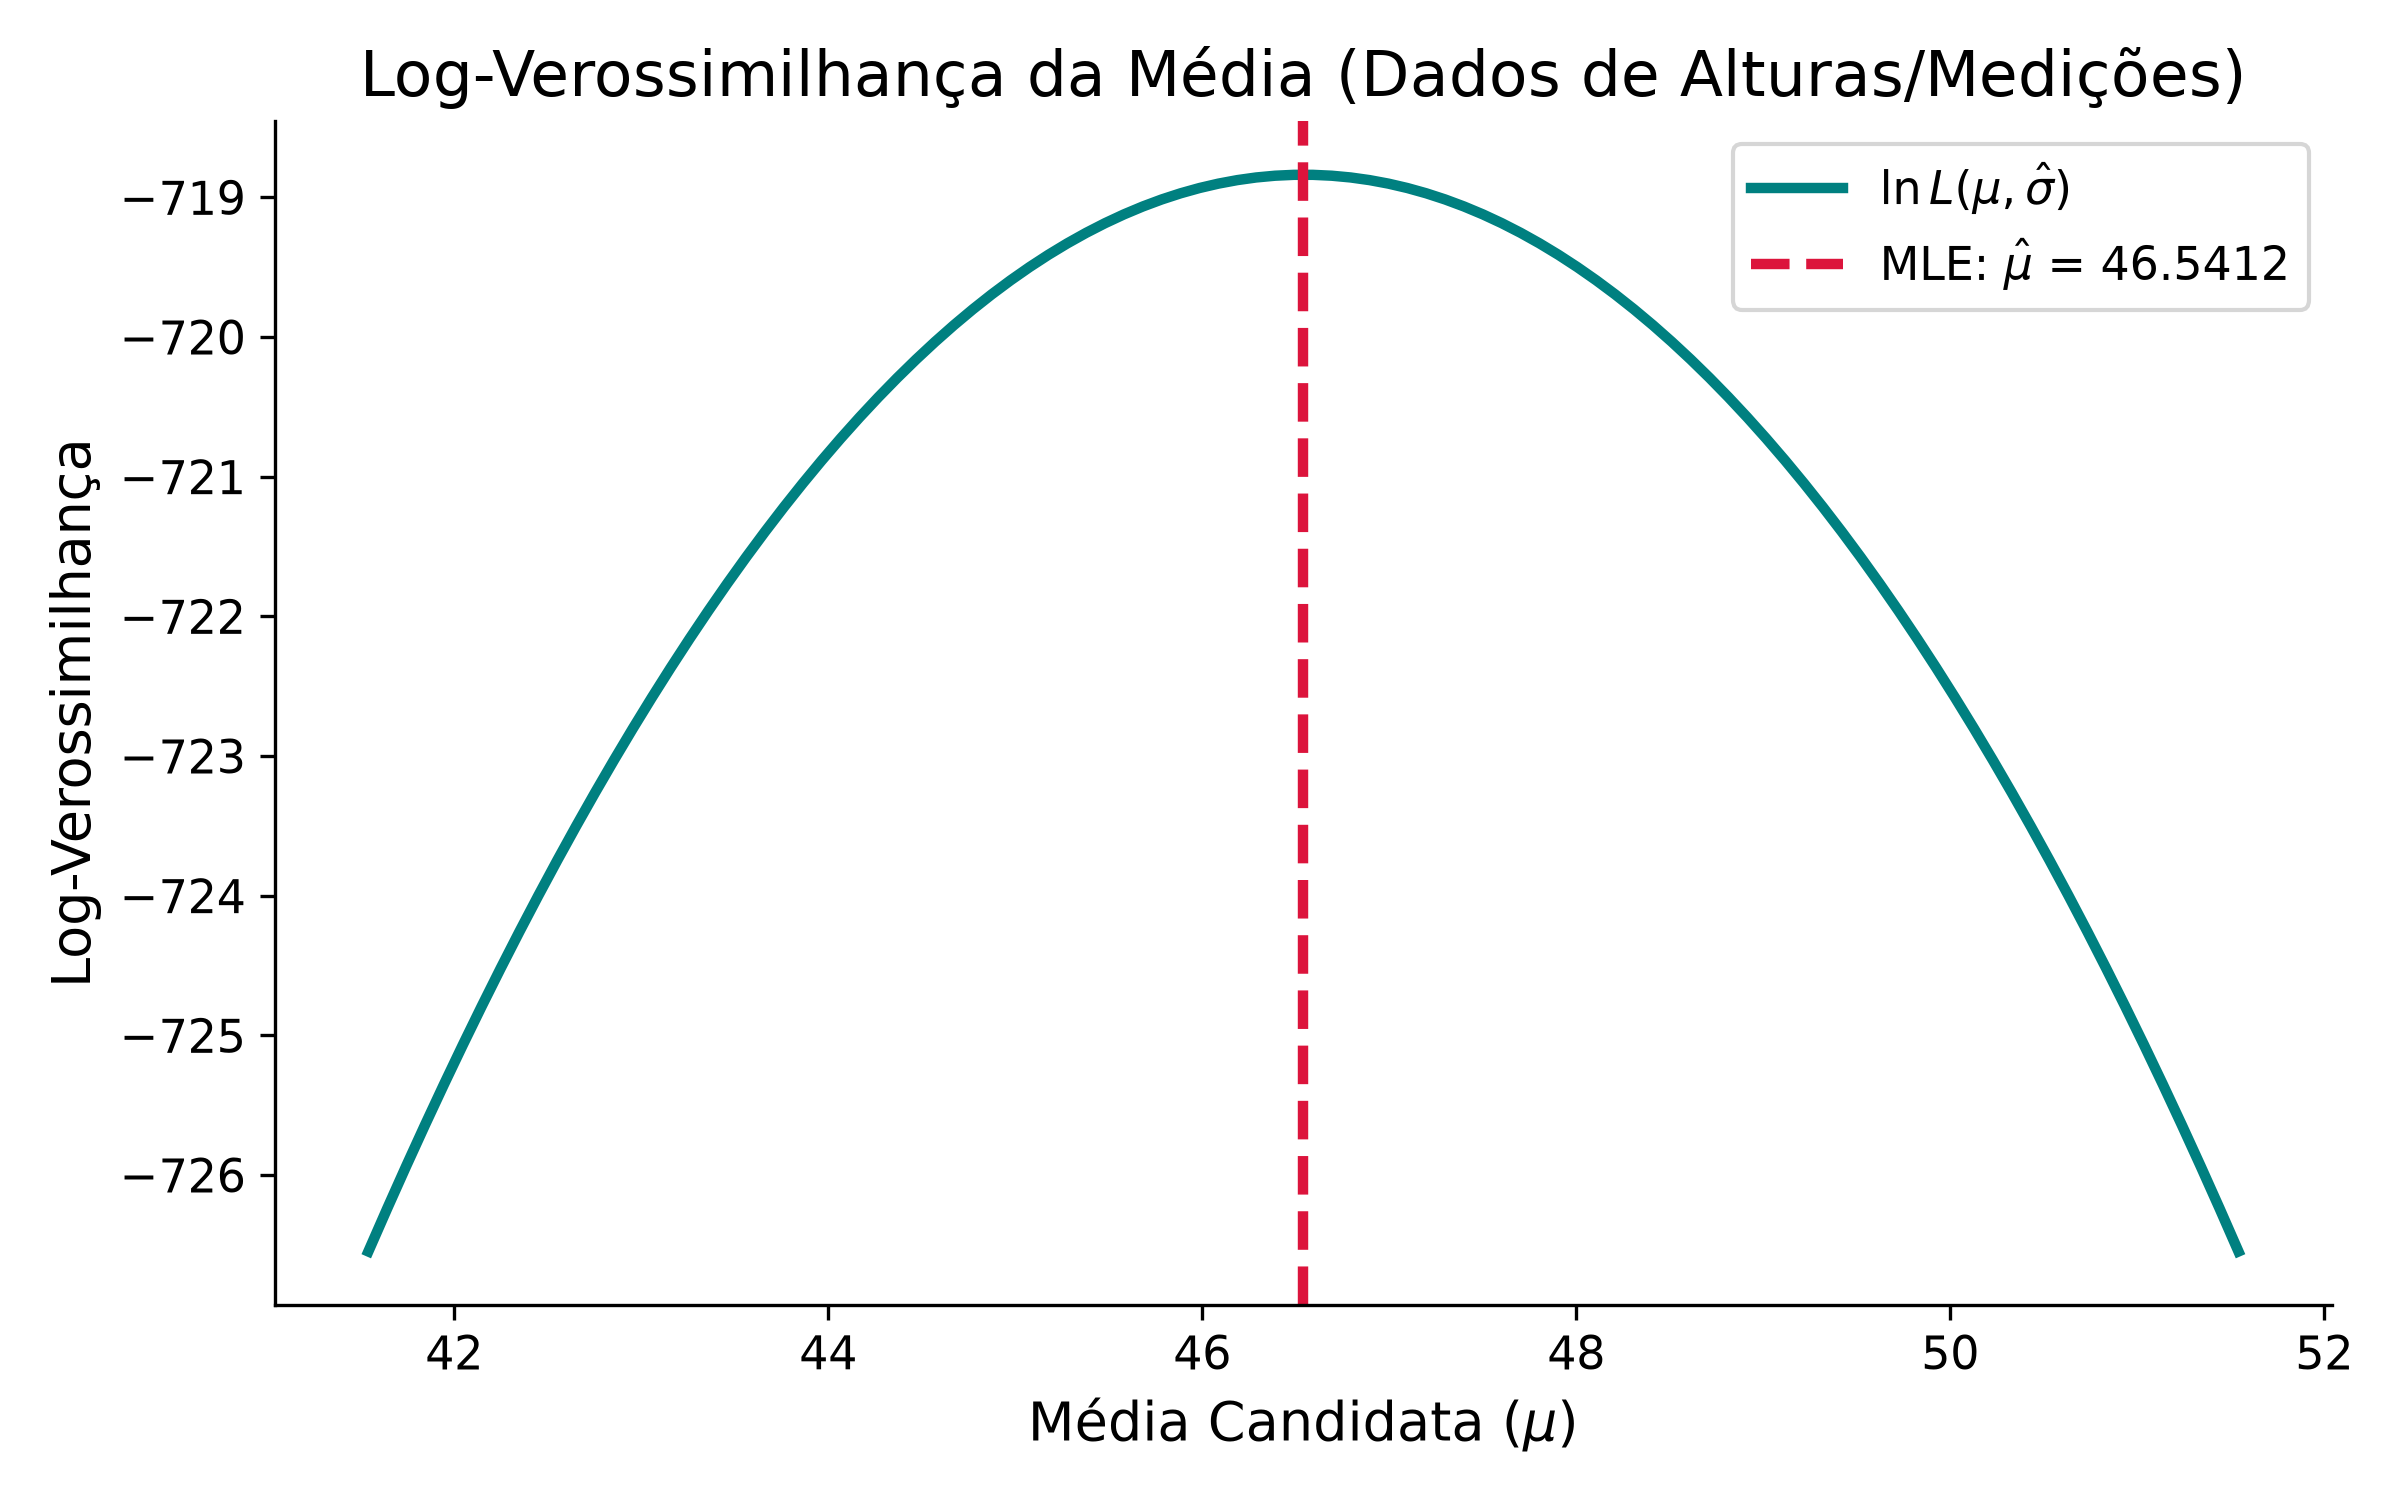
\includegraphics[width=\textwidth]{log_verossimilhanca_normal_mu.png}
        \end{column}
    \end{columns}
\end{frame}

\begin{frame}[fragile]{Exemplo Pareado: Avaliação Gaussiana}
    \begin{block}{Implementando a Log-Verossimilhança Normal em Python}
\begin{lstlisting}
import numpy as np
import scipy.stats as ss

# Amostra de medicoes
dados = np.array([41, 27, 33, 58, 24, 65, 48, 72, 36, 29, 54, 67, 21])

# Estimativas pontuais amostrais
media_amostral = np.mean(dados)
std_amostral = np.std(dados) # MLE divide por N

print(f"Media amostral: {media_amostral:.4f}")

# Funcao de log-verossimilhanca Normal usando scipy
def log_verossimilhanca_normal(dados, mu, sigma):
    pdf_valores = ss.norm.pdf(dados, loc=mu, scale=sigma)
    return np.sum(np.log(pdf_valores))

# Avaliando medias candidatas
for mu_cand in [30.0, media_amostral, 60.0]:
    ll = log_verossimilhanca_normal(dados, mu_cand, std_amostral)
    print(f"Mu candidato: {mu_cand:.4f} | Log-Verossimilhanca: {ll:.4f}")
\end{lstlisting}
    \end{block}
\end{frame}

\begin{frame}{Atividade Prática de Laboratório}
    \begin{itemize}
        \item Abra um Jupyter Notebook no ambiente do curso.
        \item \textbf{Tarefa 1 (Simulação de Moeda):}
        \begin{itemize}
            \item Simule 100 lançamentos de moeda com probabilidade $\theta = 0.65$.
            \item Implemente a função de log-verossimilhança de Bernoulli.
            \item Plote a curva de log-verossimilhança para um grid de valores candidatos e identifique o ponto de máximo.
        \end{itemize}
        \item \textbf{Tarefa 2 (Dados Gaussianos):}
        \begin{itemize}
            \item Simule 50 observações normais com média $\mu = 30$ e desvio padrão $\sigma = 5$.
            \item Crie uma função para calcular a log-verossimilhança normal.
            \item Mantenha $\sigma = 5.0$ fixo e avalie a plausibilidade para médias de 20 a 40.
            \item Verifique se o máximo numérico coincide com a média amostral observada.
        \end{itemize}
    \end{itemize}
\end{frame}
